\documentclass[
	classe=$1^{ere}STI2D$
]{évaluation}

\usepackage{diagbox}
\usepackage{tcolorbox}
\usetikzlibrary{calc}

\renewcommand{\arraystretch}{1.3}

\title{Évaluation : tableaux d'effectifs et de fréquences, probabilités}
\date{2 décembre 2022}
\author{}

\begin{document}

\maketitle

\begin{tcolorbox}
	La calculatrice est autorisée. \medskip

	Certains exercices/questions sont à faire directement sur le sujet : il faut donc le rendre avec sa copie.

	Les calculs doivent être détaillés.
\end{tcolorbox}

\begin{exercice} (sur le sujet)

	Un magasin propose des feuilles de papier. Celles-ci peuvent être épaisses ou fines, et en format A3, A4 ou A5.
	\begin{itemize}
		\item $5\%$ des feuilles fines sont en format $A3$.
		\item $20\%$ des feuilles fines sont en format $A5$.
		\item Parmi toutes les feuilles, $9\%$ sont épaisses et en format $A5$.
		\item Parmi toutes les feuilles, $76\%$ sont en format $A4$.
	\end{itemize}
	\begin{center}
		\begin{tabular}{|l|*{3}{>{\centering}p{2.2cm}|}}
			\hline
			            & fines              & épaisses            & TOTAL \tabularnewline \hline
			format $A3$ & \correction{$50$}  & \correction{$125$}  & \correction{$175$}\tabularnewline \hline
			format $A4$ & \correction{$750$} & \correction{$1150$} & \correction{$1900$} \tabularnewline \hline
			format $A5$ & \correction{$200$} & \correction{$225$}  & \correction{$425$} \tabularnewline \hline
			TOTAL       & $1000$             & $1500$              & \correction{$2500$} \tabularnewline \hline
		\end{tabular}
	\end{center}

	\begin{enumerate}
		\item Compléter le tableau ci-dessus.
		\item Quelle est l'effectif des feuilles épaisses en format $A4$ ? \correction{$1150$}
		\item Quelle est le pourcentage de feuilles $A3$ ? \correction{$\frac{175}{2500} = 7\%$}
	\end{enumerate}
\end{exercice}

\begin{exercice} (question 1 sur le sujet, le reste sur la copie)
	\begin{center}
		\begin{tabular}{|c|*{4}{>{\centering}p{1.5cm}|}}
			\hline
			\diagbox{$Y$}{$X$} & $x₁$               & $x₂$              & $x₃$               & TOTAL \tabularnewline \hline
			$y₁$               & $164$              & \correction{$78$} & $80$               & \correction{$322$}\tabularnewline \hline
			$y₂$               & $36$               & $442$             & \correction{$200$} & \correction{$678$} \tabularnewline \hline
			TOTAL              & \correction{$200$} & $520$             & $280$              & \correction{$1000$} \tabularnewline \hline
		\end{tabular}
	\end{center}

	\begin{enumerate}
		\item Compléter le tableau ci-dessus.
		\item Construire le tableaux de fréquences par rapport à l'effectif global.
		\item Donner la valeur de $f_{12}$ et $f_{23}$.
		\item Construire le tableau des fréquences conditionnelles par rapport à $x₁$.
		\item Construire le tableau des fréquences conditionnelles par rapport à $y₂$.
	\end{enumerate}
\end{exercice}

\begin{exercice} (question 1 sur le sujet, le reste sur la copie)

	Dans un avion, on trouve des passagers en $1^\text{ere}$ ou en seconde classe, et des passagers qui ont mis des bagages en soute ou non.

	On appelle $A$ l'ensemble des passagers en $1^\text{ere}$ classe, et $B$ l'ensemble des passagers ayant mis leurs bagages en soute.

	On sait que :\vspace{1em}

	\begin{minipage}{0.5\linewidth}
		\begin{itemize}
			\item Il y a $500$ passagers au total.
			\item Il y a $33$ passagers qui sont en $1^\text{ere}$ classe, et qui ont mis leurs bagages en soute.
			\item Il y a $62$ passagers qui sont en $1^\text{ere}$ classe, et qui n'ont \textbf{pas} mis leurs bagages en soute.
			\item Il y a $167$ passagers qui sont en seconde classe, et qui n'ont \textbf{pas} mis leurs bagages en soute.
		\end{itemize}
	\end{minipage}\hspace{1cm}
	\begin{minipage}{0.4\linewidth}
		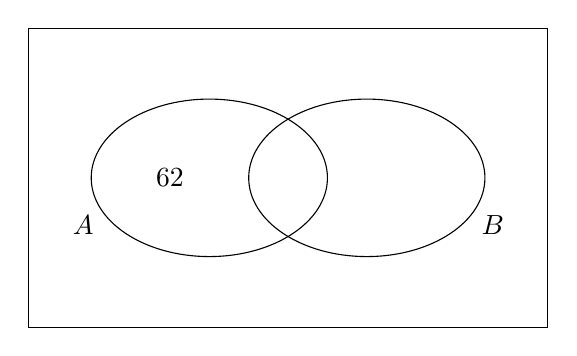
\begin{tikzpicture}
			\coordinate (A) at (-1,0);
			\coordinate (B) at (1,0);

			\draw (-3.3,-1.9) rectangle (3.3,1.9);
			\draw (A) ellipse (1.5 and 1);
			\draw (B) ellipse (1.5 and 1);
			\node at ($(A) + (-1.6,-0.6)$) {$A$};
			\node at ($(B) + (1.6,-0.6)$) {$B$};

			\node at ($(A) + (-0.5,0)$) {$62$};
			\ifdefined\makeCorrection
				\node[red] at ($(0,0)$) {$33$};
				\node[red] at ($(0,1.5)$) {$167$};
				\node[red] at ($(B) + (0.5,0)$) {$238$};
			\fi
		\end{tikzpicture}
	\end{minipage}

	\begin{enumerate}
		\item Compléter le schéma ci-dessus.
		\item Donner le cardinal de $A ∩ B$. \correction{$33$}
		\item Donner le cardinal de $\overline{A} ∩ B$. \correction{$238$}
		\item Donner le cardinal de $A ∪ B$. \correction{$62+33+238=333$}
		\item Si on prend un passager au hasard dans l'avion, quelle est la probabilité qu'il soit en seconde classe ET qu'il n'ai pas mis ses bagages en soute ? \correction{$167/500 = 0,334$}
	\end{enumerate}
\end{exercice}

\begin{exercice} (question 1 sur le sujet, le reste sur la copie)

	Une entreprise possède deux serres $A$ et $B$ qui produisent chacune deux types de fleurs (des tulipes ou des narcisses). Lors du printemps 2018, elle a vendu $350$ kg de fleurs. \medskip

	On sait que :
	\begin{itemize}
		\item Parmi toute la masse de fleurs, $72\%$ sont des tulipes.
		\item $P_{\text{Tulipes}}(\text{Serre }A) = 0,35$.
		\item $P_{\text{Narcisses}}(\text{Serre }B) = 0,8$.
	\end{itemize}

	\begin{enumerate}
		\item Compléter le tableau \textbf{d'effectifs} suivant :

		      \begin{center}
			      \begin{tabular}{|l|*{3}{>{\centering}p{2cm}|}}
				      \hline
				      \diagbox{$X =$ fleur}{$Y =$ serre} & $A$                     & $B$                     & TOTAL \tabularnewline \hline
				      Tulipe                             & \correction{$88,2$ kg}  & \correction{$163,8$ kg} & \correction{$252$ kg}\tabularnewline \hline
				      Narcisse                           & \correction{$19,6$ kg}  & \correction{$78,4$ kg}  & \correction{$98$ kg} \tabularnewline \hline
				      TOTAL                              & \correction{$107,8$ kg} & \correction{$242,2$ kg} & \correction{$350$ kg} \tabularnewline \hline
			      \end{tabular}
		      \end{center}
		\item En déduire le pourcentage de fleurs venant de la serre $A$.
		\item En déduire, parmi les fleurs de la serre $B$, le pourcentage de tulipes.
	\end{enumerate}
\end{exercice}

\begin{exercice} (sur la copie ; laisser les traces de recherches)

	On effectue un sondage parmi $300$ personnes. $15$ \% de ces personnes ont les yeux bleus, $45$ \% ont les yeux marrons, et le reste a les yeux noirs. Aucune femme n'a les yeux bleus. Deux tiers des femmes sont des fumeuses. Un cinquième des hommes sont des fumeurs. \medskip

	On choisit une personne au hasard. Sachant que la personne fume, quelle est la probabilité pour que cette personne soit une femme ?
\end{exercice}

%======================
% SUJET B
%======================
\newpage
\setcounter{exercice}{1}

\maketitle

\begin{tcolorbox}
	La calculatrice est autorisée. \medskip

	Certains exercices/questions sont à faire directement sur le sujet : il faut donc le rendre avec sa copie.

	Les calculs doivent être détaillés.
\end{tcolorbox}

\begin{exercice} (sur le sujet)

	Un magasin propose des feuilles de papier. Celles-ci peuvent être épaisses ou fines, et en format A3, A4 ou A5.
	\begin{itemize}
		\item $5\%$ des feuilles fines sont en format $A3$.
		\item $20\%$ des feuilles fines sont en format $A5$.
		\item Parmi toutes les feuilles, $9\%$ sont épaisses et en format $A5$.
		\item Parmi toutes les feuilles, $76\%$ sont en format $A4$.
	\end{itemize}
	\begin{center}
		\begin{tabular}{|l|*{3}{>{\centering}p{2.2cm}|}}
			\hline
			            & fines              & épaisses           & TOTAL \tabularnewline \hline
			format $A3$ & \correction{$40$}  & \correction{$100$} & \correction{$140$}\tabularnewline \hline
			format $A4$ & \correction{$600$} & \correction{$920$} & \correction{$1520$} \tabularnewline \hline
			format $A5$ & \correction{$160$} & \correction{$180$} & \correction{$340$} \tabularnewline \hline
			TOTAL       & $800$              & $1200$             & \correction{$2000$} \tabularnewline \hline
		\end{tabular}
	\end{center}

	\begin{enumerate}
		\item Compléter le tableau ci-dessus.
		\item Quelle est l'effectif des feuilles épaisses en format $A4$ ? \correction{$920$}
		\item Quelle est le pourcentage de feuilles $A3$ ? \correction{$\frac{140}{2000} = 7\%$}
	\end{enumerate}
\end{exercice}

\begin{exercice} (question 1 sur le sujet, le reste sur la copie)
	\begin{center}
		\begin{tabular}{|c|*{4}{>{\centering}p{1.5cm}|}}
			\hline
			\diagbox{$Y$}{$X$} & $x₁$               & $x₂$              & $x₃$               & TOTAL \tabularnewline \hline
			$y₁$               & $164$              & \correction{$78$} & $80$               & \correction{$322$}\tabularnewline \hline
			$y₂$               & $36$               & $442$             & \correction{$200$} & \correction{$678$} \tabularnewline \hline
			TOTAL              & \correction{$200$} & $520$             & $280$              & \correction{$1000$} \tabularnewline \hline
		\end{tabular}
	\end{center}

	\begin{enumerate}
		\item Compléter le tableau ci-dessus.
		\item Construire le tableaux de fréquences par rapport à l'effectif global.
		\item Donner la valeur de $f_{12}$ et $f_{23}$.
		\item Construire le tableau des fréquences conditionnelles par rapport à $x₁$.
		\item Construire le tableau des fréquences conditionnelles par rapport à $y₂$.
	\end{enumerate}
\end{exercice}

\begin{exercice} (question 1 sur le sujet, le reste sur la copie)

	Dans un avion, on trouve des passagers en $1^\text{ere}$ ou en seconde classe, et des passagers qui ont mis des bagages en soute ou non.

	On appelle $A$ l'ensemble des passagers en $1^\text{ere}$ classe, et $B$ l'ensemble des passagers ayant mis leurs bagages en soute.

	On sait que :\vspace{1em}

	\begin{minipage}{0.5\linewidth}
		\begin{itemize}
			\item Il y a $500$ passagers au total.
			\item Il y a $30$ passagers qui sont en $1^\text{ere}$ classe, et qui ont mis leurs bagages en soute.
			\item Il y a $65$ passagers qui sont en $1^\text{ere}$ classe, et qui n'ont \textbf{pas} mis leurs bagages en soute.
			\item Il y a $167$ passagers qui sont en seconde classe, et qui n'ont \textbf{pas} mis leurs bagages en soute.
		\end{itemize}
	\end{minipage}\hspace{1cm}
	\begin{minipage}{0.4\linewidth}
		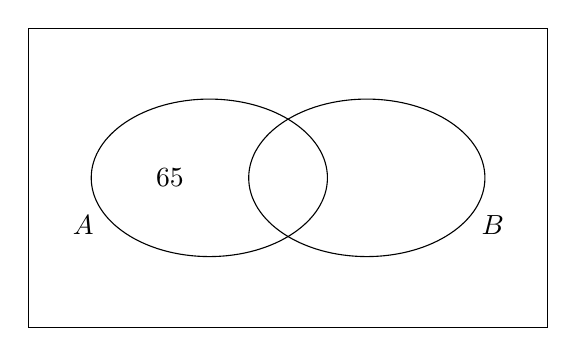
\begin{tikzpicture}
			\coordinate (A) at (-1,0);
			\coordinate (B) at (1,0);

			\draw (-3.3,-1.9) rectangle (3.3,1.9);
			\draw (A) ellipse (1.5 and 1);
			\draw (B) ellipse (1.5 and 1);
			\node at ($(A) + (-1.6,-0.6)$) {$A$};
			\node at ($(B) + (1.6,-0.6)$) {$B$};

			\node at ($(A) + (-0.5,0)$) {$65$};
			\ifdefined\makeCorrection
				\node[red] at ($(0,0)$) {$30$};
				\node[red] at ($(0,1.5)$) {$167$};
				\node[red] at ($(B) + (0.5,0)$) {$238$};
			\fi
		\end{tikzpicture}
	\end{minipage}

	\begin{enumerate}
		\item Compléter le schéma ci-dessus.
		\item Donner le cardinal de $A ∩ B$. \correction{$33$}
		\item Donner le cardinal de $\overline{A} ∩ B$. \correction{$238$}
		\item Donner le cardinal de $A ∪ B$. \correction{$62+33+238=333$}
		\item Si on prend un passager au hasard dans l'avion, quelle est la probabilité qu'il soit en seconde classe ET qu'il n'ai pas mis ses bagages en soute ? \correction{$167/500 = 0,334$}
	\end{enumerate}
\end{exercice}

\begin{exercice} (question 1 sur le sujet, le reste sur la copie)

	Une entreprise possède deux serres $A$ et $B$ qui produisent chacune deux types de fleurs (des tulipes ou des narcisses). Lors du printemps 2018, elle a vendu $350$ kg de fleurs. \medskip

	On sait que :
	\begin{itemize}
		\item Parmi toute la masse de fleurs, $72\%$ sont des tulipes.
		\item $P_{\text{Tulipes}}(\text{Serre }A) = 0,35$.
		\item $P_{\text{Narcisses}}(\text{Serre }B) = 0,8$.
	\end{itemize}

	\begin{enumerate}
		\item Compléter le tableau \textbf{d'effectifs} suivant :

		      \begin{center}
			      \begin{tabular}{|l|*{3}{>{\centering}p{2cm}|}}
				      \hline
				      \diagbox{$X =$ fleur}{$Y =$ serre} & $A$                     & $B$                     & TOTAL \tabularnewline \hline
				      Tulipe                             & \correction{$88,2$ kg}  & \correction{$163,8$ kg} & \correction{$252$ kg}\tabularnewline \hline
				      Narcisse                           & \correction{$19,6$ kg}  & \correction{$78,4$ kg}  & \correction{$98$ kg} \tabularnewline \hline
				      TOTAL                              & \correction{$107,8$ kg} & \correction{$242,2$ kg} & \correction{$350$ kg} \tabularnewline \hline
			      \end{tabular}
		      \end{center}
		\item En déduire le pourcentage de fleurs venant de la serre $A$.
		\item En déduire, parmi les fleurs de la serre $B$, le pourcentage de tulipes.
	\end{enumerate}
\end{exercice}

\begin{exercice} (sur la copie ; laisser les traces de recherches)

	On effectue un sondage parmi $300$ personnes. $15$ \% de ces personnes ont les yeux bleus, $45$ \% ont les yeux marrons, et le reste a les yeux noirs. Aucune femme n'a les yeux bleus. Deux tiers des femmes sont des fumeuses. Un cinquième des hommes sont des fumeurs. \medskip

	On choisit une personne au hasard. Sachant que la personne fume, quelle est la probabilité pour que cette personne soit une femme ?
\end{exercice}

\end{document}